% The unfolded DAG for bricks (31,41,59) and (33,83,27).
% Edge labels are the height of the brick at the destination.
% Regenerate from this directory with:
% latex -interaction=nonstopmode -halt-on-error dag-babylon.tex
% dvisvgm --no-fonts --exact --bbox=papersize -o dag-babylon.svg dag-babylon.dvi
\documentclass[tikz,border=4pt]{standalone}
\usepackage{lmodern}
\usetikzlibrary{arrows.meta,backgrounds,fit,shapes.geometric}
\definecolor{brickblue}{HTML}{337DB4}
\definecolor{repeatgold}{HTML}{C68E00}
\begin{document}
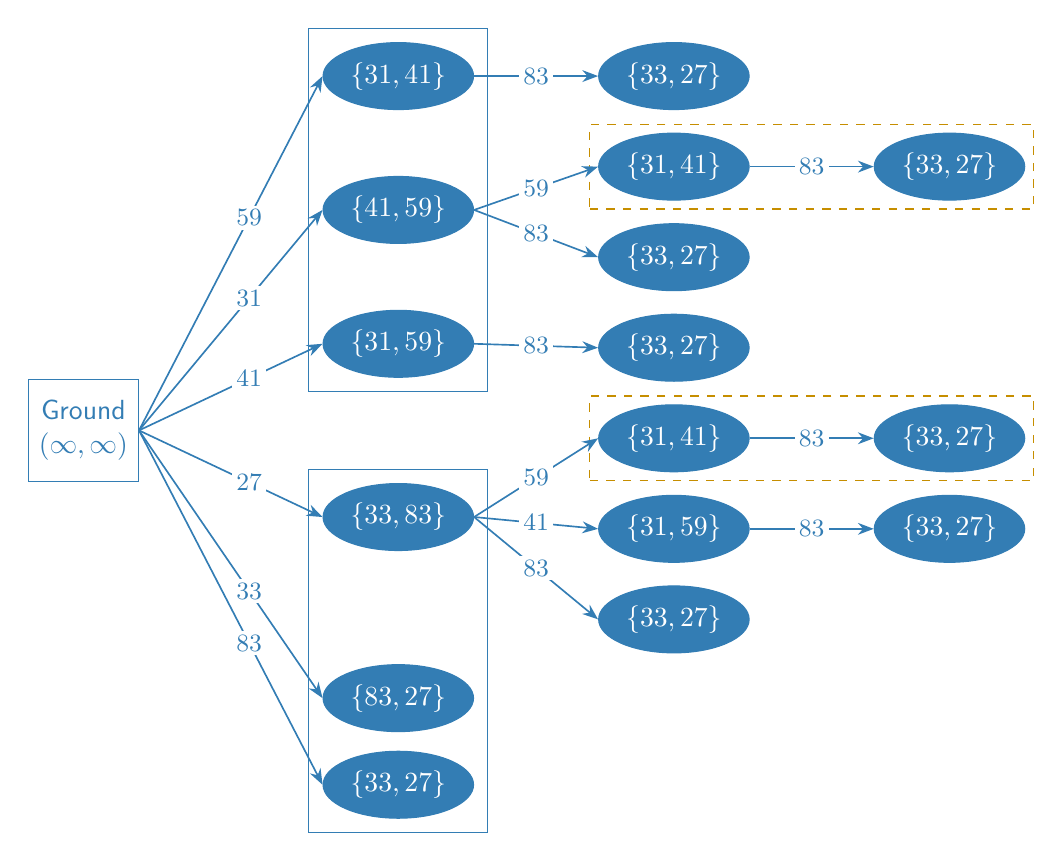
\begin{tikzpicture}[
  x=1cm,y=1cm,>=Stealth,
  brick/.style={ellipse,draw=brickblue,fill=brickblue,text=white,
    minimum width=1.65cm,minimum height=0.85cm,inner sep=2pt},
  edge/.style={->,draw=brickblue,line width=0.6pt},
  weight/.style={fill=white,inner sep=1.5pt,text=brickblue,font=\small},
  font=\sffamily
]
  \node[draw=brickblue,text=brickblue,align=center,minimum width=1.4cm,
    minimum height=1.3cm] (ground) at (0,0) {Ground\\$(\infty,\infty)$};

  % Each blue frame groups the three possible orientations of one brick.
  \node[brick] (a) at (4,4.5) {$\{31,41\}$};
  \node[brick] (b) at (4,2.8) {$\{41,59\}$};
  \node[brick] (c) at (4,1.1) {$\{31,59\}$};
  \node[brick] (d) at (4,-1.1) {$\{33,83\}$};
  \node[brick] (e) at (4,-3.4) {$\{83,27\}$};
  \node[brick] (f) at (4,-4.5) {$\{33,27\}$};

  \node[brick] (af) at (7.5,4.5) {$\{33,27\}$};
  \node[brick] (ba) at (7.5,3.35) {$\{31,41\}$};
  \node[brick] (baf) at (11,3.35) {$\{33,27\}$};
  \node[brick] (bf) at (7.5,2.2) {$\{33,27\}$};
  \node[brick] (cf) at (7.5,1.05) {$\{33,27\}$};
  \node[brick] (da) at (7.5,-0.1) {$\{31,41\}$};
  \node[brick] (daf) at (11,-0.1) {$\{33,27\}$};
  \node[brick] (dc) at (7.5,-1.25) {$\{31,59\}$};
  \node[brick] (dcf) at (11,-1.25) {$\{33,27\}$};
  \node[brick] (df) at (7.5,-2.4) {$\{33,27\}$};

  \foreach \target/\height in {a/59,b/31,c/41,d/27,e/33,f/83}
    \draw[edge] (ground.east) -- node[weight,pos=0.6] {\height} (\target.west);
  \draw[edge] (a.east) -- node[weight] {83} (af.west);
  \draw[edge] (b.east) -- node[weight] {59} (ba.west);
  \draw[edge] (b.east) -- node[weight] {83} (bf.west);
  \draw[edge] (ba.east) -- node[weight] {83} (baf.west);
  \draw[edge] (c.east) -- node[weight] {83} (cf.west);
  \draw[edge] (d.east) -- node[weight] {59} (da.west);
  \draw[edge] (d.east) -- node[weight] {41} (dc.west);
  \draw[edge] (d.east) -- node[weight] {83} (df.west);
  \draw[edge] (da.east) -- node[weight] {83} (daf.west);
  \draw[edge] (dc.east) -- node[weight] {83} (dcf.west);

  \begin{scope}[on background layer]
    \node[draw=brickblue,fit=(a)(b)(c),inner sep=5pt] {};
    \node[draw=brickblue,fit=(d)(e)(f),inner sep=5pt] {};
    \node[draw=repeatgold,dashed,fit=(ba)(baf),inner sep=3pt] {};
    \node[draw=repeatgold,dashed,fit=(da)(daf),inner sep=3pt] {};
  \end{scope}
\end{tikzpicture}
\end{document}
